\documentclass{article}
\usepackage{amsfonts}
\usepackage{amsmath}
\usepackage{amssymb}
\usepackage{color}
%\usepackage{apacite}
\usepackage{caption}
\usepackage{graphicx}
\begin{document}

\author{
  Jonsson, Haukur\\
  \texttt{11137304}
  \and
  Rajamanickam, Santhosh\\
  \texttt{11650702}
  \and
  Rapp, Max\\
  \texttt{11404310}
}
\title{A Qualitative Reasoning Model of a simple (?) Container System\\
	\large Project Report}
\maketitle



\section{Introduction}

Everyday life requires engaging with countless systems of varying complexity. Successful engagement necessitates robust approximate prediction of their behaviour. However, understanding the dynamics of even the simplest of these systems would require solving a set of differential equations of prohibitive complexity.

Rather than precise modelling, humans therefore engage in \textit{Qualitative Reasoning} to understand and predict the behaviour of systems surrounding them. Qualitative models are built by using simplifying \textit{assumptions} to construct a simplified ontology of the system including its objects and the causal relations between them as well as discretizing the quantities of the objects and the magnitudes of the relations. Such models are surprisingly powerful in predicting possible system outcomes.

It is threfore arguable that understanding a domain is a function of one's qualitative model of that domain. In this paradigm, human (and machine) learning and teaching can then be understood in terms of building and adapting qualitative models of the world. 

The computer assisted learning paradigm tries to leverage this approach by developing \textit{Human Level AI} that assists and interacts with the learner in building better qualitative models.

The goal of this project is to implement a qualitative model of a container system that could serve in an interactive learning software by taking various inputs and returning a state graph and trace of the development of the system.

\section{Two Container Models}

The system to be modelled can be described as follows: A \textbf{tap} is used to regulate the influx of water into an open \textbf{container} with a \textbf{drain} through which water escapes.

The basic ingredients needed to build a model for this system are the \textit{entities} which describe the basic objects the model contains. An entity may have one or more \textit{quantities} describing its magnitude. The quantities each have a magnitude constrained by a \textit{quantity space} containing its allowed values as well as a \textit{derivative} with quantity space (-,0,+) describing the current change in quantity. Between quantities \textit{causal relations} obtain. In our case these include \textit{influences} ($I^+$, $I^-$) and \textit{proportionalities} ($P^+$, $P^-$). Influences are positive or negative relationships from the magnitude of a quantity to the derivative of another. Proportionalities are positive or negative relationship from one derivative to another.
Another component we need are \textit{correspondences}. Correspondences can be implications or equivalences between values of quantities' magnitudes.

Using these ingredients, depending on one's assumptions, models of varying complexity of the container system can be devised. Here we describe two. 

\subsection {Model I}

\textbf{Ontology:}
\begin{itemize}
	\item Entities: Tap, Container, Drain
	\item Quantities(Spaces): Inflow (Zero; Plus), Volume (Zero, Plus, Max), Outflow (Zero, Plus, Max)
	\item Relations: $I^+$(Inflow, Volume), $I^-$(Outflow, Volume), $P^+$(Volume, Outflow)
	\item Correspondences: Volume(Zero)$\leftrightarrow$Outflow(Zero), Volume(Max)$\leftrightarrow$Outflow(Max)
\end{itemize}

The ontology above is depicted in figure \ref{fig: figure1}. To study the development of the system we not only need an ontology but also an \textit{initial state} (or \textit{scenario}). figure \ref{figure2} represents the scenario which we aim to implement for Model I. Namely, we assume that inflow and outflow are at zero in the beginning and that the inflow is exogenuously determined by a function taking the form of a positive parabola. I.e. $\delta$Inflow will initially increase but eventually stagnate and start to decrease until it reaches zero.


\begin{figure}
	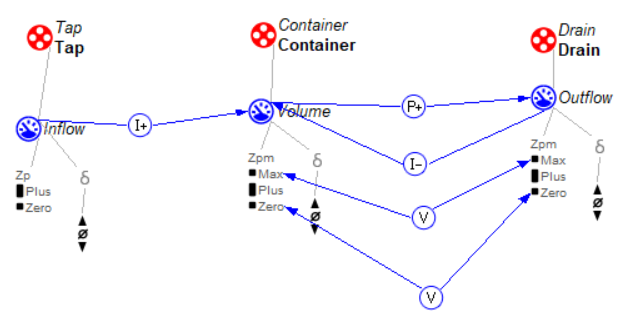
\includegraphics{Simple_Flow.png}
	\caption{Ontology of Model I. Note the red entities which indicate conditions that have to be met for the relations to apply}
	\label{fig: figure1}
\end{figure}

\begin{figure}
	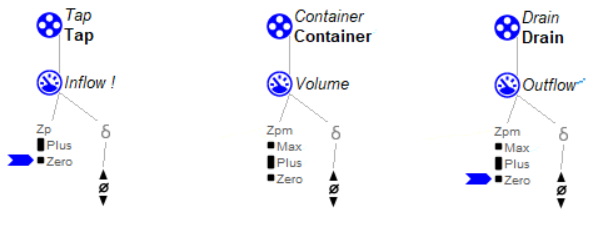
\includegraphics{Scenario_1.png}
	\caption{Initial state of Model I}
	\label{figure2}
\end{figure}

\subsection {Model II}

\textbf{Ontology:}
\begin{itemize}
	\item Entities: Tap, Container, Drain
	\item Quantities(Spaces): Inflow (Zero; Plus), Height(Zero, Plus, Max), Pressure (Zero, Plus, Max), Volume (Zero, Plus, Max), Outflow (Zero, Plus, Max)
	\item Relations: $I^+$(Inflow, Volume), $I^-$(Outflow, Volume), $P^+$(Volume, Outflow)
\end{itemize}

The more complex ontology of Model II is shown in figure \ref{figure3} and the corresponding initial state (unchanged except for entities) in figure \ref{figure4}.

\begin{figure}
	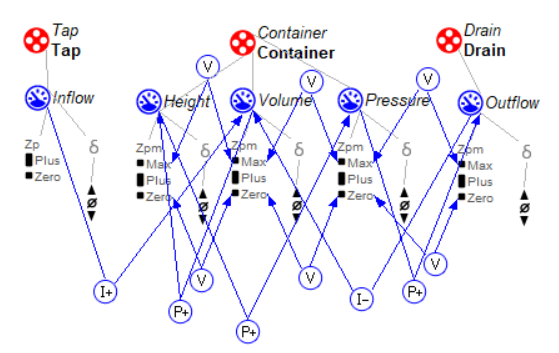
\includegraphics{Extra_Flow.png}
	\caption{In the more complex Model II, outflow is no longer determined by volume but by pressure which is in turn determined by the height of the fluid in the container which is proportiional to the volume.}
	\label{figure3}
\end{figure}

\begin{figure}
	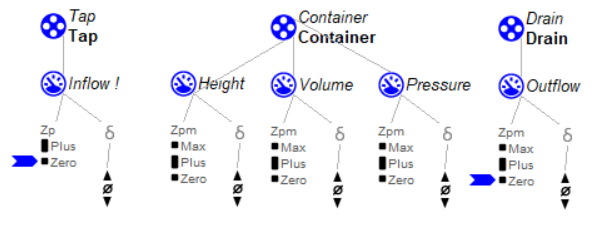
\includegraphics{Scenario_2.png}
	\caption{Initial state of Model II}
	\label{figure4}
\end{figure}

\section{Target Simulation and State Graph}

to begin with, we set up Model I and Model II in the QR-software \textit{Garp3} to create benchmarks for our implementations. Simulations using default modelling settings (figure \ref{figure5}) lead in both cases to state graphs containing 13 nodes. As expected, the unique end state (state 12 in both cases) consists of an empty container with zero in- and outflow (figure \ref{figure6}). Interestingly, the graphs of the two models look completely identical inspite of the added quantities in Model II (figure \ref{figure7}).

\begin{figure}
	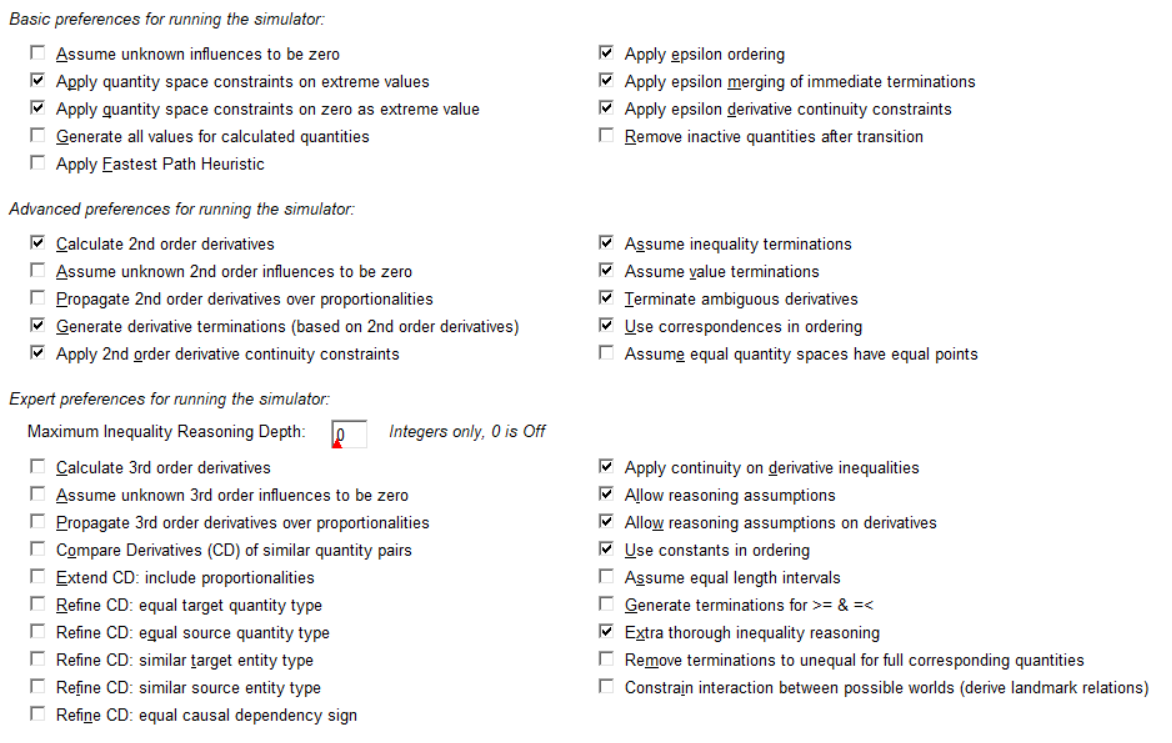
\includegraphics{Modelling_Settings}
	\caption{The modelling preferences used in our benchmark simulations.}
	\label{figure5}
\end{figure}

\begin{figure}
	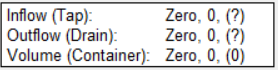
\includegraphics{End_State}
	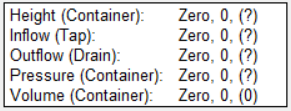
\includegraphics{End_State_Extra}
	\caption{The end states of the simulations of Model I and II respectively.}
	\label{figure6}
\end{figure}

\begin{figure}
	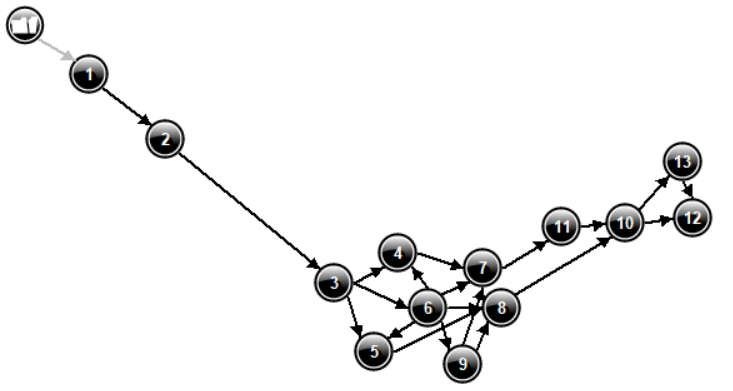
\includegraphics{Simple_State_Graph.png}
	\caption{State graph for Model I and II. While the states represented differ in the number of quantities they represent, the identity of the graph representations indicate that Model I and Model II describe the same system in two different yet - with respect to evolution - equivalent ways.}
	\label{figure7}
\end{figure}

\section{Implementation}

\subsection{Modelling Assumptions}

We now set out to recreate the state graphs of Model I and II using a much simpler implementation. Namely, of the simulation preferences described in figure \ref{figure5} we will only implement the following:


\textbf{Basic Epsilon Ordering:} Any termination that consists of a point-value changing to an interval is immediate and takes priority over changes that take time such as interval to landmark changes. \textcolor{red}{if more that one immediate terminations is applicable, ...}. In this way we divide the termination calculation into two phases \textit{static changes} and \textit{dynamic changes}. Branching can take place only in the latter phase.

\textbf{Derivative values are point values:} or equivalently proportionalities act immediately. This assumption can be justified by the fact that proportionalities are usually the result of having different descriptions of the same state of a system that are pragmatically useful but ontologically reducible to each other. In our case, consider the water column in the container in Model II: the height of the column, its volume and the pressure in the column are three different yet dependent ways of describing the same state of the system; thus if one of these quantities changes, so do the others by definition. Proportionality here thus merely describes the same change by different names and therefore acts immediately.

After inferring terminations, in a third phase, we check the consistency of the termination candidates against the following conditions:

\textbf{No magnitude change without non-zero derivative:} a magnitude of a quantity can only increase/decrease if its derivative is greater/smaller than zero. 

\textbf{No derivative change without (exogenous) influence:} likewise, we don't allow derivative changes that are not caused by an influence, proportionality or exogenous variable. 

\noindent The two preceding conditions immediately imply the next one:

\textbf{No causation by correspondence:} implications and equivalences act as sanity checks and let us throw out inconsistent states but cannot be used in the static/dynamic phases.

\textbf{No fleeting equalities:} If $I^+(A,B)$=$I^-(C,B)$ and $\delta A \neq \delta C$, $\delta B \neq 0$. The justification for this assumption is that such points of fleeting inequality should take priority by epsilon ordering since moving away from a point of equality is immediate. Therefore they should immediately terminate into a different state. However, they are not spotted by our basic epsilon ordering and hence we discard them here.

\subsection{Algorithm}

Note that these assumptions do not touch on issues such as second order derivatives or inequality reasoning. Our algorithm is thus much more primitive than Garp3's. We describe how it works by the following pseudocode:

\textcolor{red}{enter pseudocode here}

\section{Results}

Which deviations from the benchmark simulations will our modelling choices incur? And do they affect the overall degree to which our algortihm captures the behaviour of the system? 

The results of our simulations are visualized by the state graph in figure \ref{figure8} as well as the state descriptions in table \ref{table1} and \ref{table2}. Consistently with the Garp3 simulations we found that the state graphs of Model I and Model II coincide.

\begin{figure}
	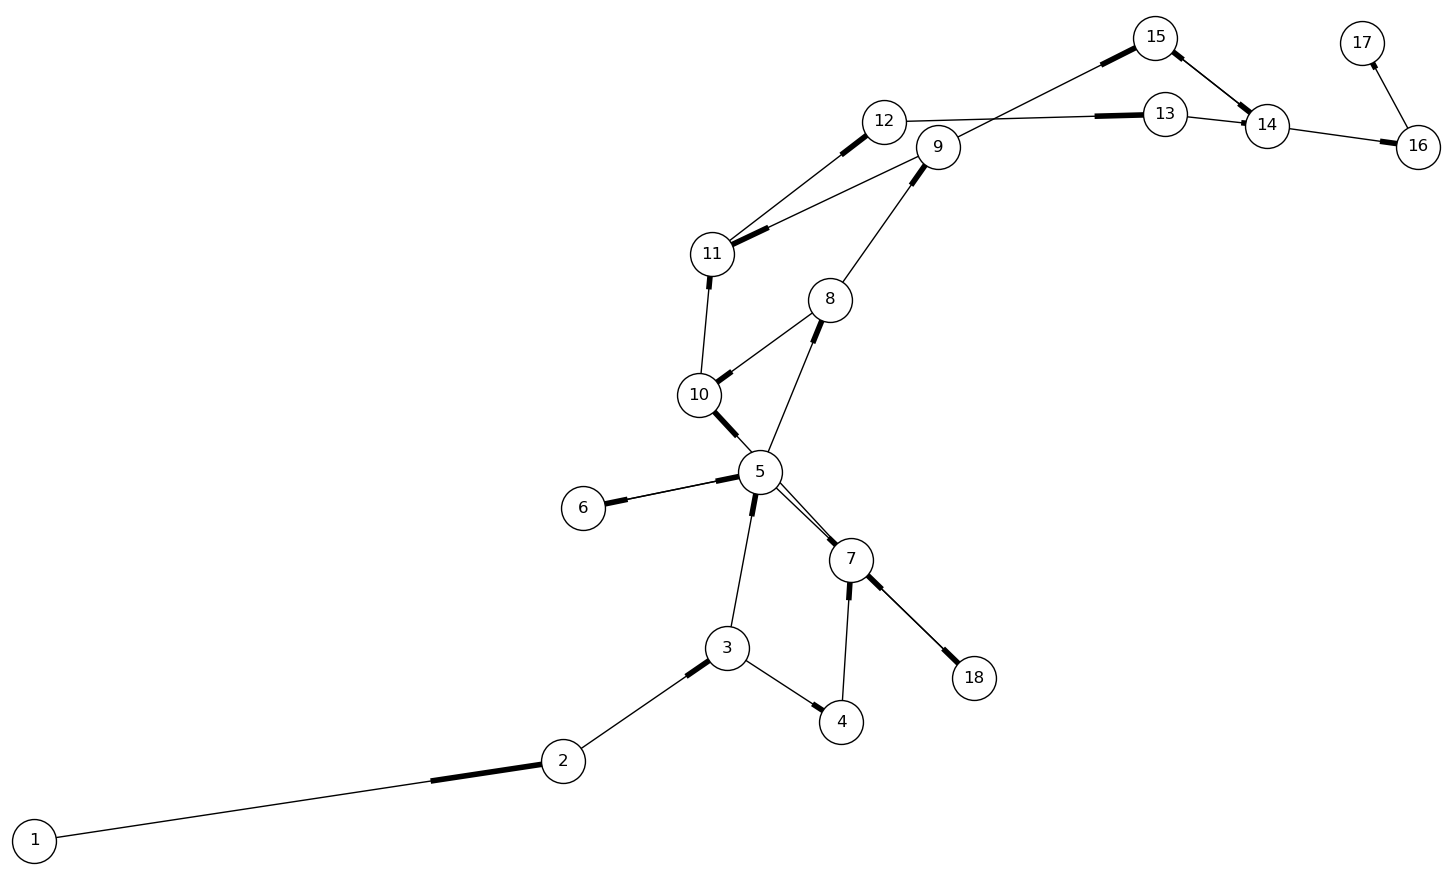
\includegraphics[scale=0.3]{Ok_State_Graph.png}
	\caption{State graph for Model I and II according to our simulation. }
	\label{figure8}
\end{figure}

\begin{table}[]
	\centering
	\caption{State table of Model I}
	\label{table1}
	\begin{tabular}{llllllll}
		\# & Inflow & $\delta$ Inflow & Volume & $\delta$ Volume & Outflow & $\delta$ Outflow & Children \\
		1  & 0      & +               & 0      & 0               & 0       & 0                & 2        \\
		2  & +      & +               & 0      & +               & 0       & +                & 3        \\
		3  & +      & +               & +      & +               & +       & +                & 4, 5     \\
		4  & +      & +               & Max    & +               & Max     & +                & 7        \\
		5  & +      & 0               & +      & +               & +       & +                & 6, 7, 8  \\
		6  & +      & 0               & +      & 0               & +       & 0                & 5        \\
		7  & +      & 0               & Max    & +               & Max     & +                & 10, 18   \\
		8  & +      & -               & +      & +               & +       & +                & 9, 10    \\
		9  & 0      & -               & +      & +               & +       & +                & 11, 15   \\
		10 & +      & -               & Max    & +               & Max     & +                & 11       \\
		11 & 0      & -               & Max    & +               & Max     & +                & 12       \\
		12 & 0      & -               & Max    & 0               & Max     & 0                & 13       \\
		13 & 0      & -               & Max    & -               & Max     & -                & 14       \\
		14 & 0      & -               & +      & -               & +       & -                & 15, 16   \\
		15 & 0      & -               & +      & 0               & +       & 0                & 14       \\
		16 & 0      & -               & 0      & -               & 0       & -                & 17       \\
		17 & 0      & -               & 0      & 0               & 0       & 0                & End      \\
		18 & +      & 0               & Max    & 0               & Max     & 0                & 7       
	\end{tabular}
\end{table}

\begin{table}[]
	\centering
	\caption{State table of Model II}
	\label{table2}
	\begin{tabular}{llllllllllll}
		\# & Inflow & $\delta$ Inflow & Height & $\delta$ Height & Pressure & $\delta$ Pressure & Volume & $\delta$ Volume & Outflow & $\delta$ Outflow & Children \\
		1  & 0      & +               &        &                 &          &                   & 0      & 0               & 0       & 0                & 2        \\
		2  & +      & +               &        &                 &          &                   & 0      & +               & 0       & +                & 3        \\
		3  & +      & +               &        &                 &          &                   & +      & +               & +       & +                & 4, 5     \\
		4  & +      & +               &        &                 &          &                   & Max    & +               & Max     & +                & 7        \\
		5  & +      & 0               &        &                 &          &                   & +      & +               & +       & +                & 6, 7, 8  \\
		6  & +      & 0               &        &                 &          &                   & +      & 0               & +       & 0                & 5        \\
		7  & +      & 0               &        &                 &          &                   & Max    & +               & Max     & +                & 10, 18   \\
		8  & +      & -               &        &                 &          &                   & +      & +               & +       & +                & 9, 10    \\
		9  & 0      & -               &        &                 &          &                   & +      & +               & +       & +                & 11, 15   \\
		10 & +      & -               &        &                 &          &                   & Max    & +               & Max     & +                & 11       \\
		11 & 0      & -               &        &                 &          &                   & Max    & +               & Max     & +                & 12       \\
		12 & 0      & -               &        &                 &          &                   & Max    & 0               & Max     & 0                & 13       \\
		13 & 0      & -               &        &                 &          &                   & Max    & -               & Max     & -                & 14       \\
		14 & 0      & -               &        &                 &          &                   & +      & -               & +       & -                & 15, 16   \\
		15 & 0      & -               &        &                 &          &                   & +      & 0               & +       & 0                & 14       \\
		16 & 0      & -               &        &                 &          &                   & 0      & -               & 0       & -                & 17       \\
		17 & 0      & -               &        &                 &          &                   & 0      & 0               & 0       & 0                & End      \\
		18 & +      & 0               &        &                 &          &                   & Max    & 0               & Max     & 0                & 7       
	\end{tabular}
\end{table}


\end{document}